\documentclass{standalone}
\usepackage[T1]{fontenc}
\usepackage[utf8]{inputenc}
\usepackage[usenames,dvipsnames]{xcolor}
\usepackage{tikz}
\usetikzlibrary{plotmarks}
\usetikzlibrary{shapes,snakes,arrows}
\begin{document}
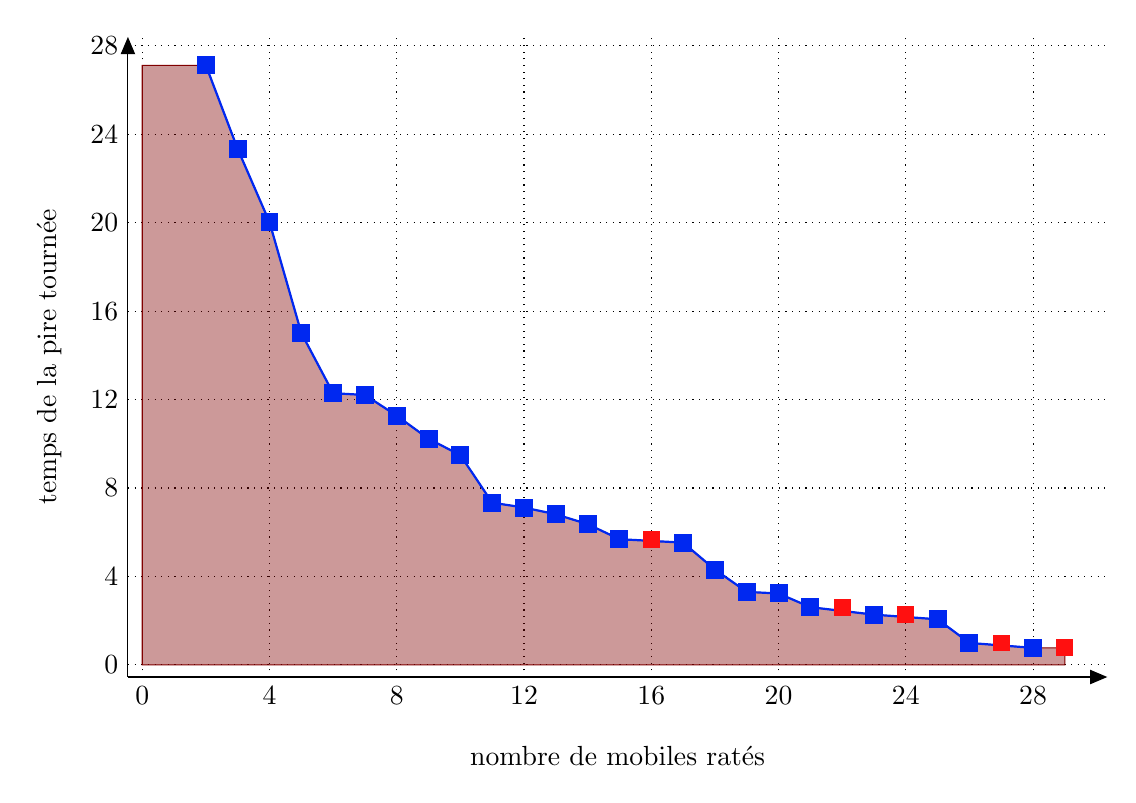
\begin{tikzpicture}[xscale=0.40404,yscale=0.28076]
\draw[xstep=4,ystep=4,thin,dotted,color=Black] (-0.45,-0.551807) grid (30.3333,28.3999);
\begin{scope}
  \clip (-0.45,-0.551807) rectangle (30.3333,28.3999);
  \definecolor{hvColor}{RGB}{128,0,0}
  \draw[color=hvColor, fill=hvColor, fill opacity=0.4]  (2,27.1168) -- (3,23.3329) -- (4,20.0216) -- (5,15.0082) -- (6,12.2862) -- (7,12.2058) -- (8,11.2678) -- (9,10.222) -- (10,9.48409) -- (11,7.33314) -- (12,7.11453) -- (13,6.80922) -- (14,6.3632) -- (15,5.6831) -- (17,5.52658) -- (18,4.30828) -- (19,3.29858) -- (20,3.22714) -- (21,2.60742) -- (23,2.26933) -- (25,2.05853) -- (26,0.989925) -- (28,0.765746) -| (29,0.765746) |- (0,0) |- cycle;
  \definecolor{pLineColor}{RGB}{128,0,0}
  \definecolor{pPointColor}{RGB}{0,40,240}
  \draw[thick,color=pPointColor] (2,27.1168) node[draw,color=pPointColor,fill=pPointColor, inner sep = 0pt, minimum size=2mm] {} -- (3,23.3329) node[draw,color=pPointColor,fill=pPointColor, inner sep = 0pt, minimum size=2mm] {} -- (4,20.0216) node[draw,color=pPointColor,fill=pPointColor, inner sep = 0pt, minimum size=2mm] {} -- (5,15.0082) node[draw,color=pPointColor,fill=pPointColor, inner sep = 0pt, minimum size=2mm] {} -- (6,12.2862) node[draw,color=pPointColor,fill=pPointColor, inner sep = 0pt, minimum size=2mm] {} -- (7,12.2058) node[draw,color=pPointColor,fill=pPointColor, inner sep = 0pt, minimum size=2mm] {} -- (8,11.2678) node[draw,color=pPointColor,fill=pPointColor, inner sep = 0pt, minimum size=2mm] {} -- (9,10.222) node[draw,color=pPointColor,fill=pPointColor, inner sep = 0pt, minimum size=2mm] {} -- (10,9.48409) node[draw,color=pPointColor,fill=pPointColor, inner sep = 0pt, minimum size=2mm] {} -- (11,7.33314) node[draw,color=pPointColor,fill=pPointColor, inner sep = 0pt, minimum size=2mm] {} -- (12,7.11453) node[draw,color=pPointColor,fill=pPointColor, inner sep = 0pt, minimum size=2mm] {} -- (13,6.80922) node[draw,color=pPointColor,fill=pPointColor, inner sep = 0pt, minimum size=2mm] {} -- (14,6.3632) node[draw,color=pPointColor,fill=pPointColor, inner sep = 0pt, minimum size=2mm] {} -- (15,5.6831) node[draw,color=pPointColor,fill=pPointColor, inner sep = 0pt, minimum size=2mm] {} -- (17,5.52658) node[draw,color=pPointColor,fill=pPointColor, inner sep = 0pt, minimum size=2mm] {} -- (18,4.30828) node[draw,color=pPointColor,fill=pPointColor, inner sep = 0pt, minimum size=2mm] {} -- (19,3.29858) node[draw,color=pPointColor,fill=pPointColor, inner sep = 0pt, minimum size=2mm] {} -- (20,3.22714) node[draw,color=pPointColor,fill=pPointColor, inner sep = 0pt, minimum size=2mm] {} -- (21,2.60742) node[draw,color=pPointColor,fill=pPointColor, inner sep = 0pt, minimum size=2mm] {} -- (23,2.26933) node[draw,color=pPointColor,fill=pPointColor, inner sep = 0pt, minimum size=2mm] {} -- (25,2.05853) node[draw,color=pPointColor,fill=pPointColor, inner sep = 0pt, minimum size=2mm] {} -- (26,0.989925) node[draw,color=pPointColor,fill=pPointColor, inner sep = 0pt, minimum size=2mm] {} -- (28,0.765746) node[draw,color=pPointColor,fill=pPointColor, inner sep = 0pt, minimum size=2mm] {};
  \definecolor{pLineColor}{RGB}{255,16,16}
  \definecolor{pPointColor}{RGB}{255,16,16}
  \node[draw,color=pPointColor,fill=pPointColor, inner sep = 0pt, minimum size=2mm] at (16,5.6831) {};
  \node[draw,color=pPointColor,fill=pPointColor, inner sep = 0pt, minimum size=2mm] at (22,2.60742) {};
  \node[draw,color=pPointColor,fill=pPointColor, inner sep = 0pt, minimum size=2mm] at (24,2.26933) {};
  \node[draw,color=pPointColor,fill=pPointColor, inner sep = 0pt, minimum size=2mm] at (27,0.989925) {};
  \node[draw,color=pPointColor,fill=pPointColor, inner sep = 0pt, minimum size=2mm] at (29,0.765746) {};
\end{scope}
\draw[->,>=triangle 45] (-0.45,-0.551807) -- coordinate (x axis mid) (30.3333,-0.551807);
\node[below=1cm,anchor=center] at (x axis mid) {nombre de mobiles ratés};
\foreach \x in {0,4,8,12,16,20,24,28}
  \draw (\x,-0.551807) -- (\x,-0.551807) node[anchor=north] {\x};
\draw[->,>=triangle 45] (-0.45,-0.551807) -- coordinate (y axis mid) (-0.45,28.3999);
\node[left=1cm,rotate=90,anchor=center] at (y axis mid) {temps de la pire tournée};
\foreach \y in {0,4,8,12,16,20,24,28}
  \draw (-0.45,\y) -- (-0.45,\y) node[anchor=east] {\y};
\end{tikzpicture}
\end{document}
